\section{The second Deformation Lemma}

\begin{remark}
   In the following, whenever talking about homology, it will be the homology
   with coefficients in $\R$.
\end{remark}

\begin{theorem}[Second deformation Lemma, Milnor]
   \label{theorem:2nd deformation lemma}
   Let $M$ be a manifold, $f: M \rightarrow \R$ smooth and $p$ be a 
   non-degenerate critical point of $f$ of index $\lambda$. Let $c := f(p)$ and 
   $\varepsilon > 0$, s.th. $f^{-1}[c-\varepsilon, c+\varepsilon]$ is compact 
   and contains no critical points of $f$ other then $p$. Then 
   $M^{c+\varepsilon}$ has the homotopy-type of  $M^{c-\varepsilon}$ with a 
   $\lambda$-cell attached.
\end{theorem}
 
\begin{proof}
   The idea of the proof is define a new function $F$, that is equal to $f$
   exept for in a small neighborhood of $p$, there we take $F < f$ slightly. 
   Then we get a situation as in the following diagram, where our manifold is
   the Torus and the map is the hight map, where $c = f(p)$:

   \begin{figure}[H]
      \centering
      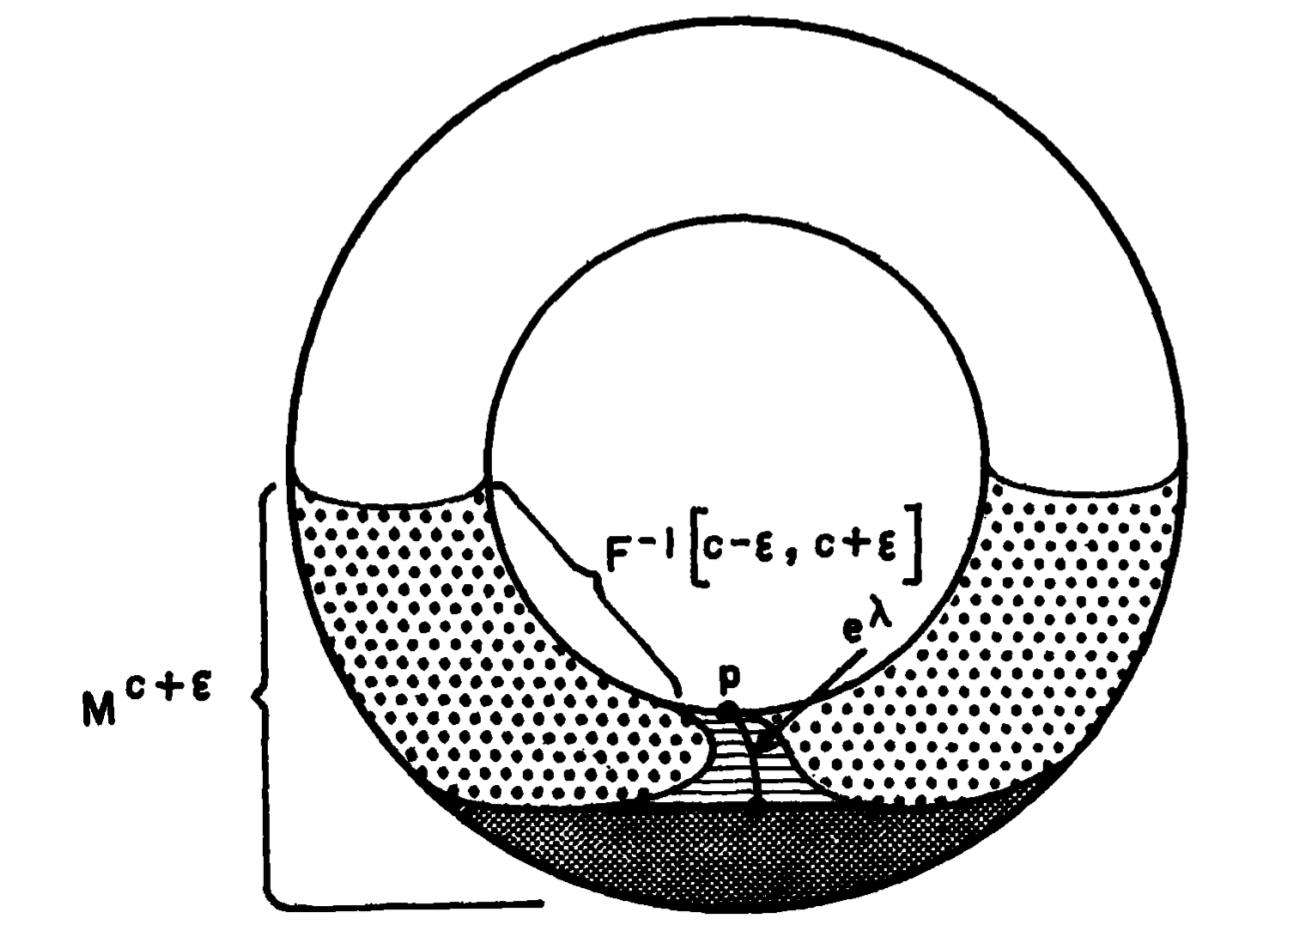
\includegraphics[width=0.5\linewidth]{resources/Mil-Diagram4.png}
      \label{fig:mil-diagram4}
   \end{figure}

   The heavily shaded region is $M^{c-\varepsilon}$. Then $F^{-1}(-\infty, c]$ is
   the heavily shaded region together with the horizontally shaded region. We Then
   construct a homotopy-equivalence that "squishes" the horizontally shaded region
   along the indicated lines, thus only leaving a $\lambda$-cell.

   By the Morse Lemma \ref{theorem:morse lemma}, we can choose local coordinates
   $\varphi = (u^1, ..., u^n)$ in a neighborhood of $p$ such that 
   \[ f = c -  (u^1)^2 - ... - (u^{\lambda})^2 + (u^{\lambda + 1})^2 + ... + (u^n)^2 \]
   in a neighborhood $U$ of $p$. Then for the critical point $p$ we have
   \[ u^1(p) = ... = u^n(p) = 0 \]
   Now choose $\varepsilon > 0$ small enough, such that the following two 
   statements hold:
   \begin{enumerate}
      \item $f^{-1}[c - \varepsilon, c + \varepsilon]$ is compact and contains
         no critical points of $f$.
      \item $\{ x: \lVert x \rVert \leq 2\varepsilon \} \subseteq \varphi(U)$
   \end{enumerate}

   Now choose the $\lambda$-cell $e^{\lambda}$ to be the points in M with
   \[ (u^1)^2 + ... + (u^{\lambda})^2 \leq \varepsilon 
   \text{ and } u^{\lambda + 1} = ... = u^n = 0 \].

   We now have our mainfold parametrized in $U$ in a nice way. The situation is
   illustrated in the following diagram:

   \begin{figure}[H]
      \centering
      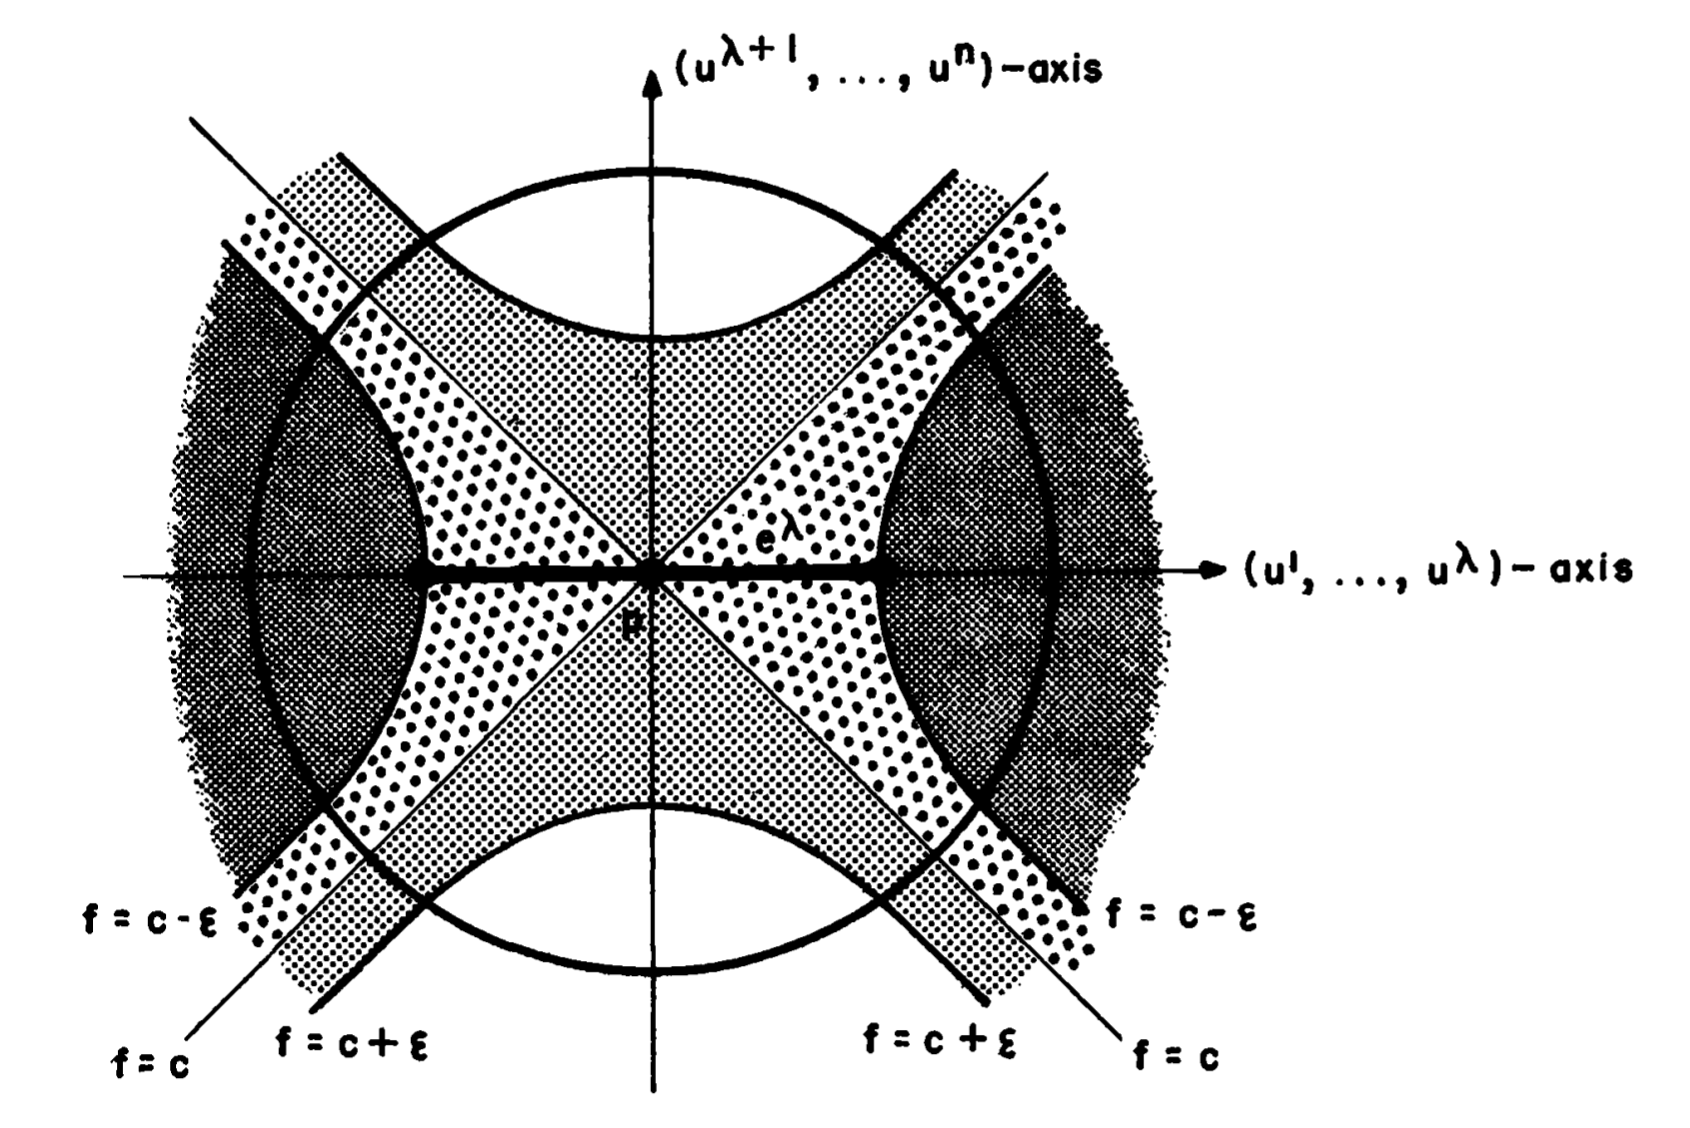
\includegraphics[width=0.7\linewidth]{resources/Mil-Diagram5.png}
      \label{fig:mil-diagram5}
   \end{figure}

   The heavily shaded area is $M^{c-\varepsilon}$, the area shaded with bigger
   dots is $f^{-1}[c - \varepsilon, c]$ and the area shaded with smaller dots
   is $f^{-1}[c, c + \varepsilon]$. \\
   The circle is $\{ p \in M : (u^1(p))^2 + ... + (u^n(p))^2 = 2\varepsilon \}$.
   Notice that $e^\lambda \cap M^{c - \varepsilon} = \del e^{\lambda}$, so
   it is attached to $M^{c - \varepsilon}$ as required. We now have to show that
   $e^{\lambda} \cup M^{c - \varepsilon}$ is a deformation retract of 
   $M^{c + \varepsilon}$. \\
   Define a $C^{\infty}$ function $\mu : \R \rightarrow \R$ with the following
   properties:
   \begin{align*}
      & \mu(0) > \varepsilon \\
      & \mu(r) = 0 \text{ for } r \geq 2\varepsilon \\
      & -1 < \mu'(r) \leq 0 \text{ for all } r
   \end{align*}

   Now let $F$ equal $f$ outside of $U$, and let 
   \[ F = f - \mu((u^1)^2 + ... + (u^{\lambda})^2 + 2(u^{\lambda + 1})^2 + ... + 2(u^n)^2) \]
   within $U$. $F$ is well defined and smooth, because for 
   $ ((u^1)^2 + ... + (u^n)^2)(p) > 2\varepsilon $, $\mu(p) = 0$ and the closed
   ball with radius $\sqrt{2\varepsilon}$ is fully contained in $U$. \\
   Now define 
   \[ \xi, \eta: U \rightarrow [0, \infty) \]
   by
   \begin{align*}
      & \xi = (u^1)^2 + ... + (u^{\lambda})^2 \\
      & \eta = (u^{\lambda + 1})^2 + ... + (u^n)^2
   \end{align*}
   Then $f = c - \xi + \eta$ and $F|_U = f - \mu(\xi + 2\eta) = c - \xi + \eta - \mu(\xi + 2\eta)$

   Assertion 1: The region $F^{-1}(-\infty, c + \varepsilon]$ coincides with 
   $M^{c + \varepsilon}$.

   For $\xi(p) + 2 \eta(p) > 2 \varepsilon$, $f(p) = F(p)$. So wlog., 
   let $p \in M$ such that $\xi(p) + 2 \eta(p) \leq 2 \varepsilon$. Then 
   \[ F(p) \leq f(p) = c + \xi(p) + \eta(p) 
   \leq c + \frac{1}{2} \xi(p) + \eta(p) 
   \leq c + \varepsilon \]. 
   This prooves the first assertion.

   Assertion 2: The critical points of $F$ are the same as those of $f$.

   Note that 
   \[ \pderive[F]{\xi} = -1 - \mu'(\xi + 2 \eta) < 0\]
   and
   \[ \pderive[F]{\eta} = 1 - 2 \mu'(\xi + 2 \eta) \geq 1 \]
   , so in particular these derivatives are never $0$. Since 
   \[ \opd F = \pderive[F]{\xi}\opd\xi + \pderive[F]{\eta} \opd \eta \]
   And d$\xi$ and d$\eta$ are zero only in $p$, $F$ has no critical points
   in $U$ other then $p$. This proves the second assertion.

   Assertion 3: The region $F^{-1}(-\infty, c - \varepsilon]$ is a deformation 
   retract of $M^{c + \varepsilon}$.

   Consider the region $F^{-1}[c - \varepsilon, c + \varepsilon]$. With 
   assertion 1 and the fact that $F \leq f$, we see that
   \[ F^{-1}[c - \varepsilon, c + \varepsilon] \subseteq f^{-1}[c - \varepsilon, c + \varepsilon] \] .
   But $f^{-1}[c - \varepsilon, c + \varepsilon]$ is compact and 
   $F^{-1}[c - \varepsilon, c + \varepsilon]$ is closed, so it is compact as 
   well. By assertion 2, it cannot contain any critical points of $F$ exept 
   maybe $p$, but
   \[ F(p) = c - \mu(0) < c - \varepsilon \],
   so $p$ is not in the region. Then with the first deformation 
   lemma~\ref{theorem:1st deformation lemma}, the third assertion is proven.
   
   In the following, $H$ will be the closure of 
   $F^{-1}(- \infty, c - \varepsilon] - M^{c - \varepsilon}$, which we shall 
   call a "handle". So $F^{-1}(- \infty, c - \varepsilon] = M^{c - \varepsilon} \cup H$
   will be called "$M^{c - \varepsilon}$ with a handle attached".

   Now consider $e^{\lambda}$ from above, i.e. the $\lambda$-cell consisting of
   all points $q$ with
   \[ \xi(q) \leq \varepsilon \text{ and } \eta(q) = 0 \].
   Since $\pderive[F]{\xi} < 0$, we have
   \[ F(q) \leq F(p) < c - \varepsilon \],
   but $f(q) \geq c - \varepsilon$ for $q \in e^{\lambda}$, so $e^{\lambda}$ 
   is contained in the handle $H$.

   Assertion 4: $M^{c - \varepsilon} \cup e^{\lambda}$  is a deformation 
   retract of $M^{c - \varepsilon} \cup H$.

   We construct a deformation retraction 
   $r: M^{c - \varepsilon} \cup H \times [0, 1] \rightarrow M^{c - \varepsilon} \cup H$ 
   for $q$ as follows:

   \[ 
      r(q, t) = \begin{cases}
         \varphi^{-1} \circ (u^1, ..., u^{\lambda}, tu^{\lambda + 1}, ..., tu^n) (q) 
               & \text{ if } \xi(q) \leq \varepsilon \\
         \varphi^{-1} \circ (u^1, ..., u^{\lambda}, s_tu^{\lambda + 1}, ..., s_tu^n) (q) 
               & \text { if } \varepsilon \leq \xi(q) \leq \eta(q) + \varepsilon \\
         q & \text{ if } \eta(q) + \varepsilon \leq \xi(q)
      \end{cases}
   \]

   Where 

   \[ s_t = t + (1 - t)((\xi - \varepsilon)/\eta)^{1/2} \]

   We have:
   
   \begin{itemize}
      \item[] $\xi(p) \leq \varepsilon$ as case 1,
      \item[] $\varepsilon \leq \xi(q) \leq \eta(q) + \varepsilon$ as case 2 and
      \item[] $\eta(q) + \varepsilon \leq \xi(q)$ case 3.
   \end{itemize}
   
   Note that 
   \[ \text{case 3, i.e. } \eta(q) + \varepsilon \leq \xi(q)
   \Leftrightarrow c - \xi(q) + \eta(q) \leq c - \varepsilon 
   \Leftrightarrow q \in M^{c - \varepsilon}\]
   , so we have the following situation:

   \begin{figure}[H]
      \centering
      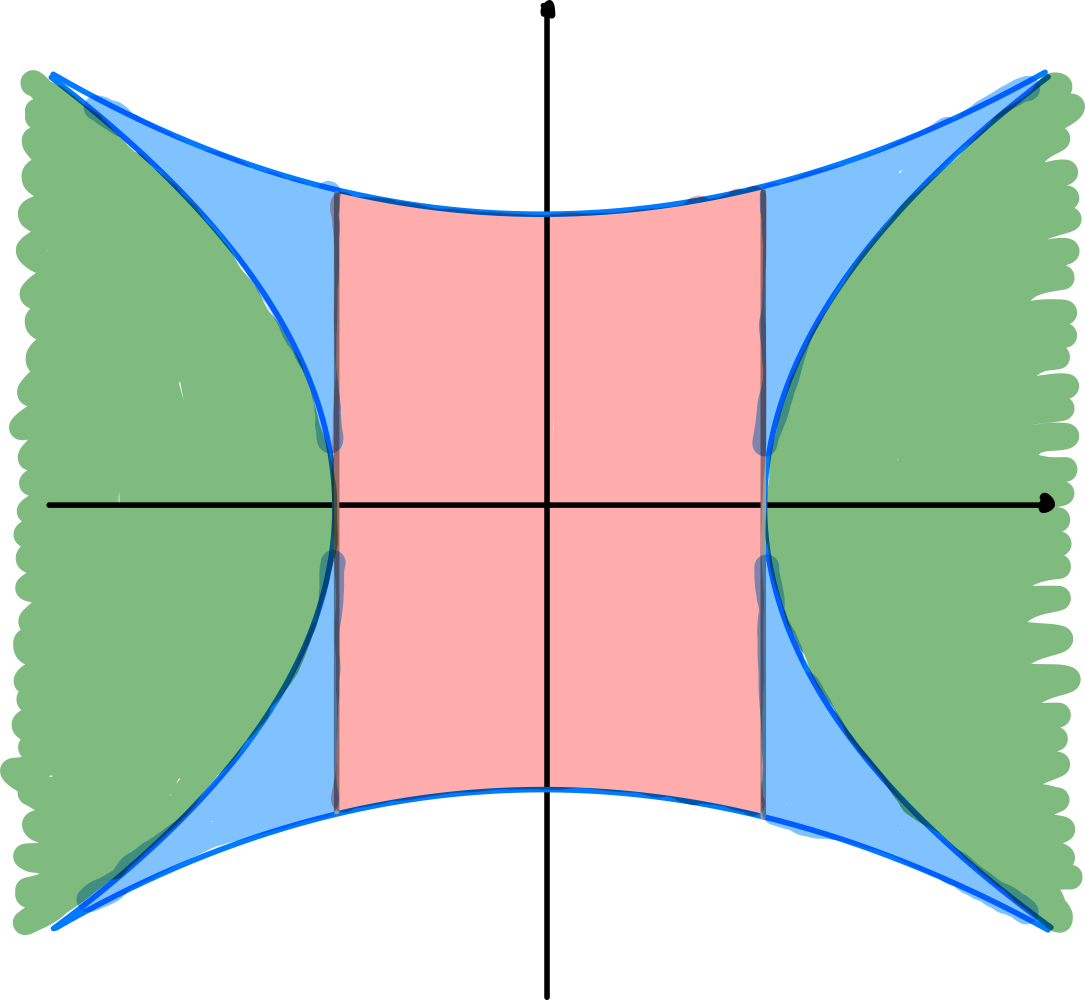
\includegraphics[width=0.6\linewidth]{./resources/Me-Diagram1.jpeg}
   \end{figure}

   Where the red is case 1, the green is case 3 and the blue is case 2.
   We now need to verify that
   \begin{enumerate}
      \item $r$ is well definded and continuous 
      \item $r(\cdot, 1) = \id_{M^{c - \varepsilon} \cup H}$
      \item $r(M^{c - \varepsilon} \cup H, 0) 
         \subseteq M^{c - \varepsilon} \cup e^{\lambda}$
      \item $r(\cdot, 0)|_{M^{c - \varepsilon} \cup e^{\lambda}} 
         = \id_{M^{c - \varepsilon} \cup e^{\lambda}}$
   \end{enumerate}

   2. and 4. are easiliy verified:
   $s_1 = 1$, so in all three cases $r(q, 1) = q$. If $q$ is in $e^{\lambda}$,
   only case 1 will hold for $q$ and then 
   $r(q, 0) = \varphi^{-1} \circ (u^1, ..., u^{\lambda}, 0, ..., 0) \in e^{\lambda}$,
   and if $q \in M^{c - \varepsilon}$ then only case 3 holds for $q$ and 
   $r(q, 0) = q \in M^{c - \varepsilon}$.

   3. is obvious for case 1 and case 3. For $q$ in case 2:
   \[ s_0(q) = ((\xi(q) - \varepsilon)/\eta(q))^{1/2} \]
   so
   \[
      f(r(0, q)) = 
         f(\varphi^{-1})(u^1(q), ... , u^{\lambda}(q), 
            \left( \frac{\xi(q) - \varepsilon}{\eta(q)} \right)^{1/2} u^{\lambda + 1}(q), ... , 
            \left( \frac{\xi(q) - \varepsilon}{\eta(q)} \right)^{1/2} u^n(q)) 
   \]
   \[
      = c - \xi(q) + \left( \left( \frac{\xi(q) - \varepsilon}{\eta(q)} \right)^{1/2} u^{\lambda + 1} \right)^2
         + \left( \left( \frac{\xi(q) - \varepsilon}{\eta(q)} \right)^{1/2} u^n(q) \right)^2
   \]
   \[ = c - \xi(q) + \left( \frac{\xi(q) - \varepsilon}{\eta(q)} \right)\eta(q) \]
   \[ = c - \varepsilon \]
   , so $r(0, q) \in f^{-1}(c - \varepsilon)$.

   To check 1. well definedness and continuity, we first need to check 
   continuity on the edge cases: 
   \begin{align*}
      & \text{For } \xi(q) = \varepsilon \text{ : } 
         & s_t(q) = t + (1 - t)((\varepsilon - \varepsilon)/\eta(q))^{1/2} = t \\
      & \text{For } \eta(q) + \varepsilon = \xi(q) \text{ : }
         & s_t(q) = t + (1 - t)((\xi(q) - \varepsilon)/(\xi(q) - \varepsilon)^{1/2} 
         = 1
   \end{align*}

   Check continuity of $s_t$:
   The only problem we may get is if $\eta \rightarrow 0$. Note that, because 
   $s_t$ is only defined in case 2, we always have $0 \leq \xi - \varepsilon \leq \eta$. 
   Then we will have to verify that $s_tu^i \rightarrow 0$ for $\lambda + 1 \leq i \leq n$,
   as $\eta \rightarrow 0$, because 
   $r(t, q) = \varphi^{-1} \circ (u^1, ..., u^{\lambda}, 0, ..., 0)$ in the other
   two cases as $\eta = 0$.

   \begin{align*}
      \lim\limits_{\eta \to 0} | s_t u^i |
         & = \lim\limits_{\eta \to 0} (1 - t)((\xi - \varepsilon)/\eta)^{1/2} | u^i | \\
         & \leq \lim\limits_{\eta \to 0} (1 - t)(\eta/\eta)^{1/2}|u^i| \\
         & = \lim\limits_{\eta \to 0} (1 - t)|u^i| = 0 
   \end{align*}

   And then $\lim\limits_{\eta \to 0} s_t u^i = 0$.
   
   Assertions 3. and 4. together prove the theorem because we get 
   \[ M^{c + \varepsilon} \simeq M^{c-\varepsilon} \cup H \]
   by assertion 3 and
   \[ M^{c-\varepsilon} \cup H \simeq M^{c - \varepsilon} \cup e^{\lambda} \]
   by assertion 4, so $M^{c + \varepsilon} \simeq M^{c - \varepsilon} \cup e^{\lambda}$.
 \end{proof}

\begin{remark}[Milnor]
   More generally, suppose there are $k$ critical points $p_1, ..., p_k$ with 
   indicies $\lambda_1, ..., \lambda_k$ in $f^{-1}(c)$. Then by a similar proof
   we get
   \[ 
      M^{c + \varepsilon} \simeq 
      M^{c - \varepsilon} \cup e^{\lambda_1} \cup ... \cup e^{\lambda_k} 
   \]
\end{remark}

\begin{remark}[Milnor]
   A simple modification of the proof above shows that $M^c$ is also a deformation
   retract $M^{c + \varepsilon}$. In fact $M^c$ is a deformation retract of 
   $F^{-1}(-\infty, c]$, which is a deformation retract of $M^{c + \varepsilon}$.
   Combinining this fact with The second deformation 
   lemma~\ref{theorem:2nd deformation lemma}, we can easily see that 
   $M^{c - \varepsilon}$ is a deformation retract of $M^c$.
\end{remark}
